% =====================================================================
%  Chapitre 11 : Permissions
% =====================================================================
\chapter{Les permissions et la sécurité}
\label{ch:permissions}

\chapitreresume{Un site de bibliothèque accueille des publics différents : les
lecteurs consultent et empruntent, les bibliothécaires gèrent le catalogue, les
administrateurs configurent le site. Dans ce chapitre, vous mettez en place des
groupes, des permissions et des contrôles d'accès. Vous découvrez aussi les
réglages de sécurité que tout projet Django doit activer avant la mise en ligne.}

\begin{objectifs}
\begin{itemize}
  \item Comprendre les permissions automatiques créées par Django.
  \item Créer des groupes et leur attribuer des droits.
  \item Vérifier une permission dans une vue fonction et une vue classe.
  \item Afficher ou masquer un élément avec \code{perms} dans un gabarit.
  \item Déclarer une permission personnalisée.
  \item Distinguer permission globale et permission objet.
  \item Appliquer les réglages de sécurité essentiels.
  \item Éviter les erreurs classiques de contrôle d'accès.
\end{itemize}
\end{objectifs}

\section{Pourquoi des permissions ?}

L'authentification répond à la question \og qui êtes-vous ? \fg. L'autorisation
répond à \og avez-vous le droit de faire ceci ? \fg. Un utilisateur connecté n'est
pas forcément autorisé à supprimer un livre.

\begin{retenir}
Une permission est un droit nommé, par exemple \code{catalogue.add\_livre}. Django
crée automatiquement quatre permissions pour chaque modèle : ajouter, modifier,
supprimer et voir. Les groupes rassemblent des permissions pour les attribuer
facilement à plusieurs utilisateurs.
\end{retenir}

\begin{figure}[htbp]
\centering
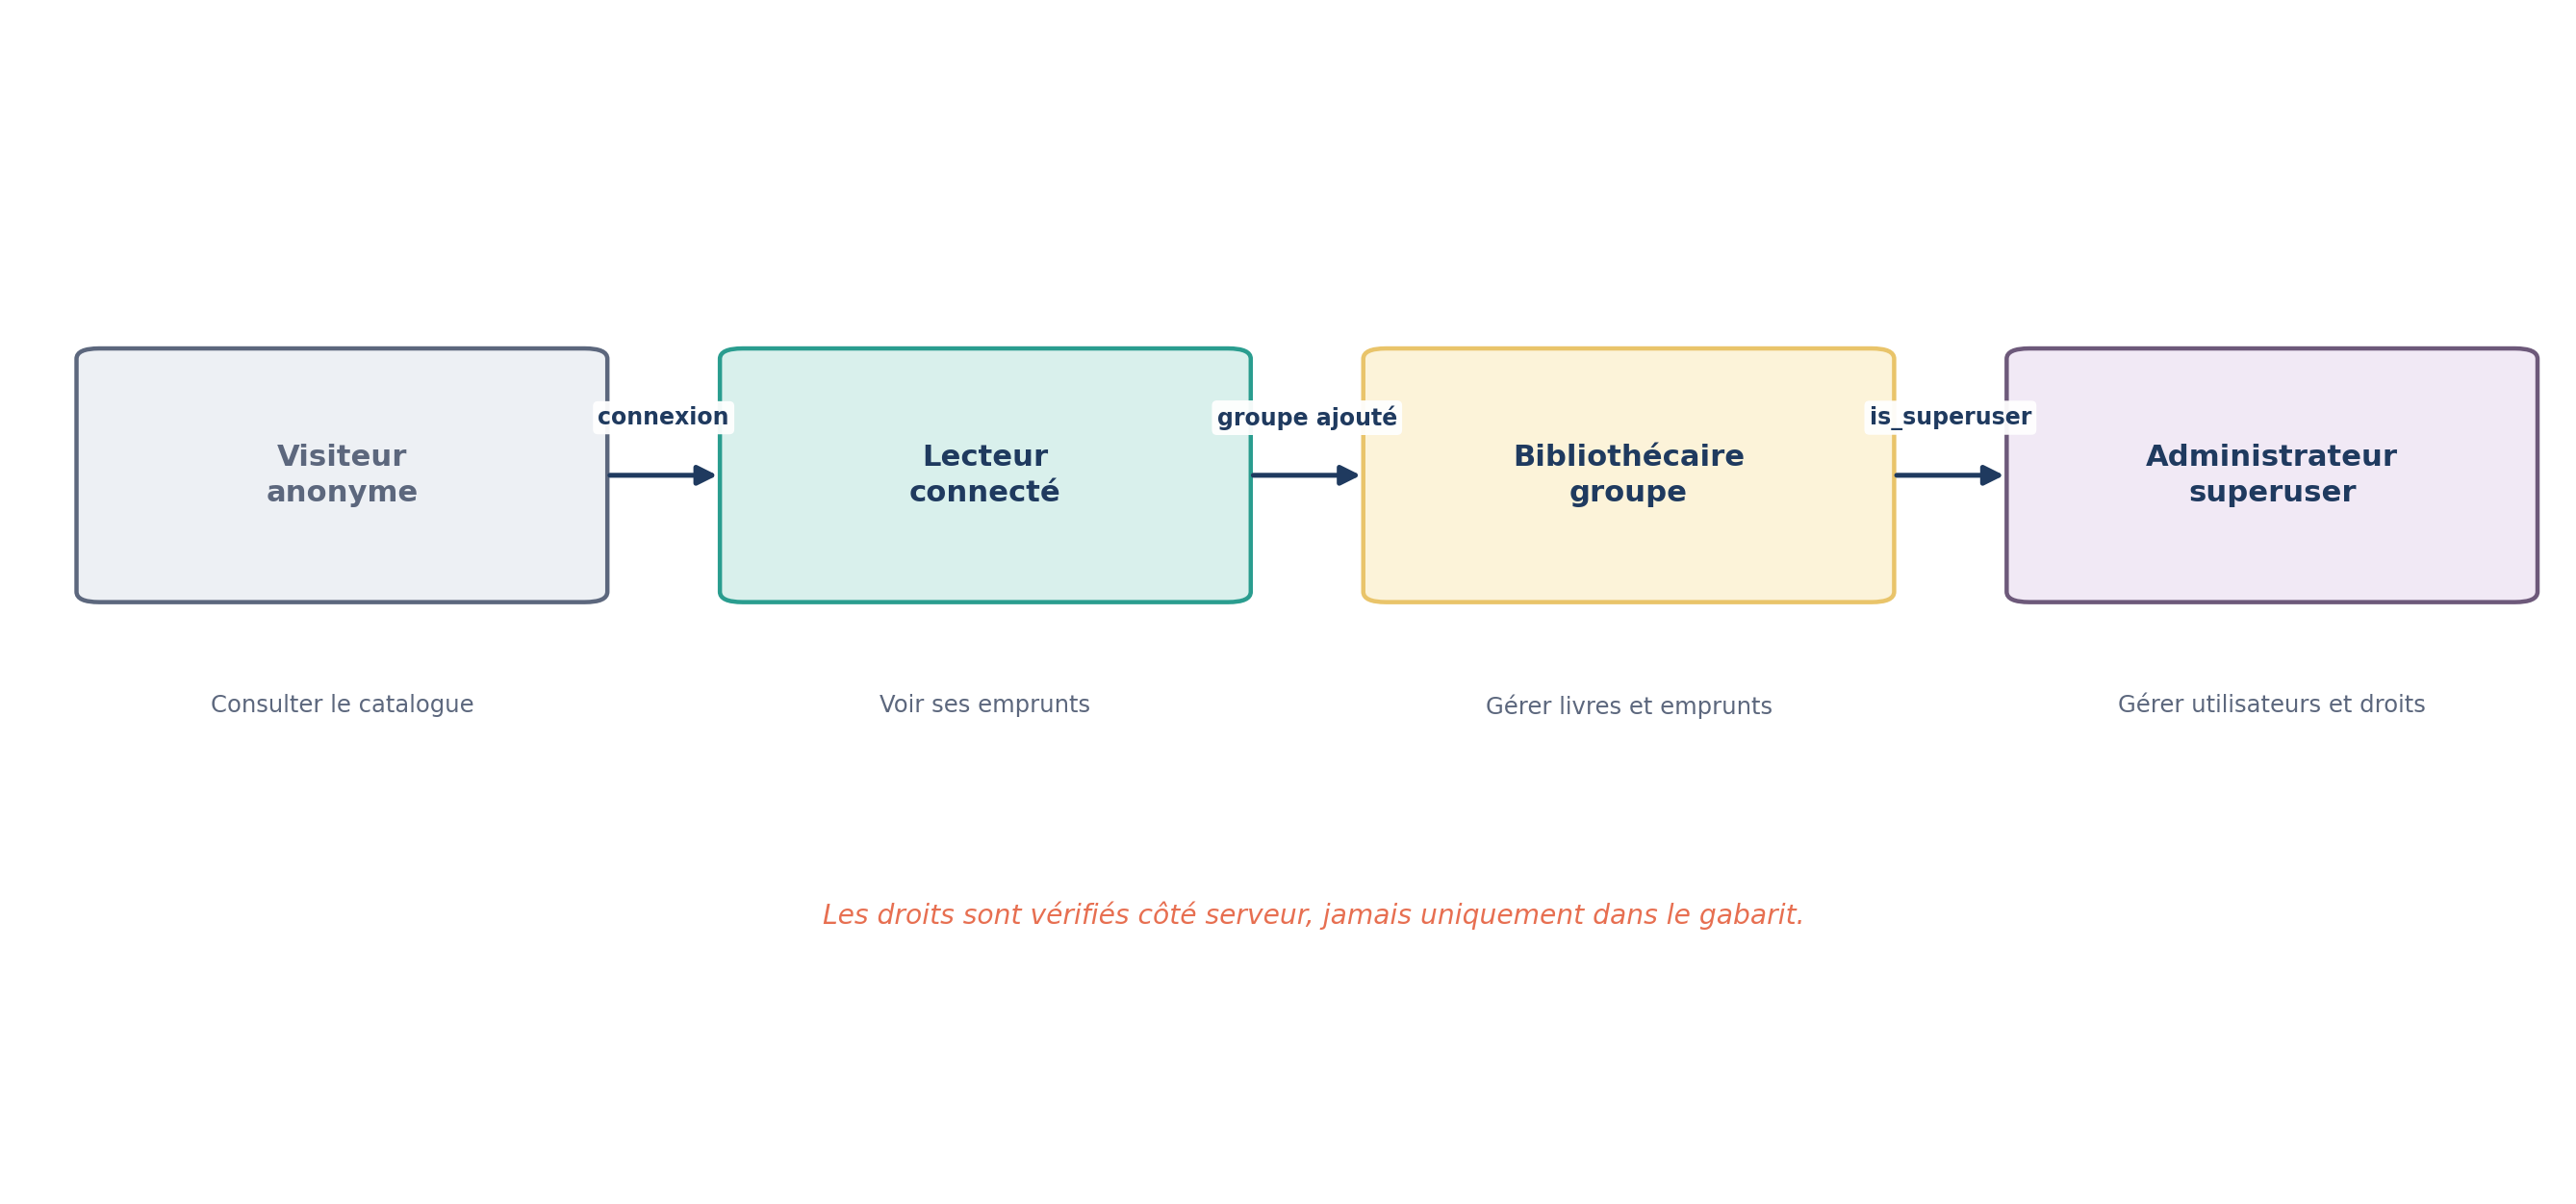
\includegraphics[width=\textwidth]{images/permissions.png}
\caption{Les utilisateurs reçoivent des groupes ; les groupes portent des
permissions ; le contrôle s'effectue dans la vue et dans le gabarit.}
\label{fig:permissions}
\end{figure}

\section{Les permissions automatiques}

Pour chaque modèle, Django crée quatre permissions :

\begin{table}[htbp]
\centering
\small
\begin{tabularx}{\textwidth}{L{4.9cm} L{3.1cm} X}
\toprule
\textbf{Codename} & \textbf{Modèle} & \textbf{Droit} \\
\midrule
\code{add\_livre} & Livre & Ajouter un livre. \\
\code{change\_livre} & Livre & Modifier un livre. \\
\code{delete\_livre} & Livre & Supprimer un livre. \\
\code{view\_livre} & Livre & Consulter un livre. \\
\bottomrule
\end{tabularx}
\caption{Les quatre permissions créées pour le modèle Livre.}
\end{table}

Le nom complet d'une permission combine l'application et le nom court de
l'action, par exemple \code{catalogue.change\_livre}. Les permissions sont
créées lors de \code{migrate}, puis mises à jour à chaque migration.

\begin{codebox}[python]{Lire les permissions d'un utilisateur}
user.has_perm("catalogue.add_livre")
user.has_perm("catalogue.delete_livre")
user.get_all_permissions()
user.get_group_permissions()
user.is_superuser   # True : toutes les permissions
\end{codebox}

\begin{note}
Un superutilisateur réussit toujours \code{has\_perm}, même sans permission
explicite. Un membre du personnel (\code{is\_staff}) n'a pas automatiquement de
droits sur les modèles : il peut seulement accéder à l'interface
d'administration. Les deux notions sont distinctes.
\end{note}

\section{Créer des groupes}

Les groupes se gèrent dans l'administration, section \og Groupes \fg. Pour
\gesibiblio, nous créons deux groupes :

\begin{table}[htbp]
\centering
\small
\begin{tabularx}{\textwidth}{L{4.1cm} X}
\toprule
\textbf{Groupe} & \textbf{Permissions} \\
\midrule
\code{Lecteurs} & \code{view\_livre}, \code{view\_auteur},
\code{view\_categorie}, \code{add\_emprunt}, \code{view\_emprunt} \\
\code{Bibliothécaires} & Toutes les permissions du catalogue, sauf la suppression
des emprunts. \\
\bottomrule
\end{tabularx}
\caption{Groupes proposés pour GesiBiblio.}
\end{table}

\begin{bonne}
Attribuez les permissions aux groupes, pas aux utilisateurs un par un. Quand un
nouveau bibliothécaire arrive, il suffit de l'ajouter au groupe. Quand une
permission change, tous les membres du groupe en bénéficient immédiatement.
\end{bonne}

On peut aussi créer les groupes par script, dans une migration de données ou une
commande de gestion. Voici une commande simple :

\begin{codebox}[python]{catalogue/management/commands/creer\_groupes.py}
from django.contrib.auth.models import Group, Permission
from django.core.management.base import BaseCommand


class Command(BaseCommand):
    help = "Crée les groupes et permissions de GesiBiblio."

    def handle(self, *args, **options):
        lecteurs, _ = Group.objects.get_or_create(name="Lecteurs")
        bibliothecaires, _ = Group.objects.get_or_create(
            name="Bibliothécaires"
        )

        codes_lecteurs = [
            "view_livre",
            "view_auteur",
            "view_categorie",
            "add_emprunt",
            "view_emprunt",
        ]
        codes_biblio = [
            "add_livre",
            "change_livre",
            "delete_livre",
            "view_livre",
            "add_auteur",
            "change_auteur",
            "add_categorie",
            "change_categorie",
            "view_emprunt",
            "change_emprunt",
            "view_membre",
        ]

        lecteurs.permissions.set(
            Permission.objects.filter(
                content_type__app_label="catalogue",
                codename__in=codes_lecteurs,
            )
        )
        bibliothecaires.permissions.set(
            Permission.objects.filter(
                content_type__app_label="catalogue",
                codename__in=codes_biblio,
            )
        )

        self.stdout.write(self.style.SUCCESS("Groupes créés."))
\end{codebox}

\begin{terminal}
python manage.py creer_groupes
\end{terminal}

\begin{attention}
Le dossier \code{management/commands/} doit contenir des fichiers
\code{\_\_init\_\_.py} à chaque niveau. Sans eux, Django ne découvre pas la
commande et affiche \code{Unknown command}.
\end{attention}

\section{Vérifier une permission dans une vue}

\subsection{Le décorateur permission\_required}

\begin{codebox}[python]{Protéger une vue fonction}
from django.contrib.auth.decorators import (
    login_required,
    permission_required,
)


@login_required
@permission_required("catalogue.add_livre", raise_exception=True)
def livre_creer(request):
    ...
\end{codebox}

\begin{description}[leftmargin=4.9cm,style=nextline]
  \item[\code{login\_required}] Redirige un visiteur non connecté vers la
  connexion.
  \item[\code{permission\_required}] Vérifie la permission. Sans
  \code{raise\_exception}, l'utilisateur connecté mais non autorisé est redirigé
  vers la connexion, ce qui est déroutant.
  \item[\code{raise\_exception=True}] Renvoie une erreur \code{403 Forbidden},
  plus correcte pour un utilisateur authentifié.
\end{description}

\begin{attention}
L'ordre des décorateurs compte. Placez \code{login\_required} au-dessus de
\code{permission\_required} pour que le visiteur soit d'abord authentifié. Dans
tous les cas, utilisez \code{raise\_exception=True} : un utilisateur connecté sans
droit doit recevoir une 403, pas une page de connexion.
\end{attention}

\subsection{Le mixin PermissionRequiredMixin}

\begin{codebox}[python]{Protéger une vue classe}
from django.contrib.auth.mixins import (
    LoginRequiredMixin,
    PermissionRequiredMixin,
)
from django.views.generic import CreateView

from .forms import LivreForm
from .models import Livre


class LivreCreateView(
    LoginRequiredMixin,
    PermissionRequiredMixin,
    CreateView,
):
    model = Livre
    form_class = LivreForm
    template_name = "catalogue/livres/formulaire.html"
    permission_required = "catalogue.add_livre"
    raise_exception = True
\end{codebox}

\begin{attention}
L'ordre d'héritage est important : \code{LoginRequiredMixin} puis
\code{PermissionRequiredMixin} puis la vue générique. Si vous inversez, le contrôle
peut être court-circuité. \code{permission\_required} accepte aussi une liste de
permissions, auquel cas toutes sont exigées.
\end{attention}

\section{Les permissions dans les gabarits}

Le processeur de contexte \code{auth} expose \code{perms}. On peut ainsi masquer un
bouton que l'utilisateur ne peut pas utiliser.

\begin{codebox}[html]{Afficher selon les droits}
{% if perms.catalogue.add_livre %}
  <a class="bouton bouton-principal"
     href="{% url 'catalogue:livre_creer' %}">Ajouter un livre</a>
{% endif %}

{% if perms.catalogue.change_livre %}
  <a class="bouton"
     href="{% url 'catalogue:livre_modifier' livre.slug %}">Modifier</a>
{% endif %}

{% if perms.catalogue.delete_livre %}
  <a class="bouton bouton-danger"
     href="{% url 'catalogue:livre_supprimer' livre.slug %}">Supprimer</a>
{% endif %}
\end{codebox}

\begin{attention}
Masquer un bouton dans le gabarit ne protège rien. Un utilisateur peut saisir
l'URL directement. La vérification du gabarit améliore l'expérience ; la vraie
protection est dans la vue. Faites toujours les deux.
\end{attention}

\begin{bonne}
Le nom dans le gabarit suit la forme \code{perms.<application>.<codename>}. Ici,
\code{perms.catalogue.add\_livre}. Vérifiez l'orthographe exacte dans
l'administration, section permissions : une faute de frappe masque silencieusement
le bouton, sans provoquer d'erreur.
\end{bonne}

\section{Une permission personnalisée}

Les quatre permissions automatiques ne suffisent pas toujours. Par exemple,
\og valider un emprunt \fg{} ou \og exporter le catalogue \fg{} sont des actions
propres au métier.

\begin{codebox}[python]{catalogue/models.py, extrait}
class Livre(models.Model):
    # ... champs existants

    class Meta:
        # ... options existantes
        permissions = [
            ("peut_marquer_perdu", "Peut marquer un livre comme perdu"),
            ("peut_exporter_catalogue", "Peut exporter le catalogue"),
        ]
\end{codebox}

Après \code{makemigrations} et \code{migrate}, les permissions apparaissent dans
l'administration. On les vérifie ainsi :

\begin{codebox}[python]{Vérifier une permission personnalisée}
@permission_required(
    "catalogue.peut_marquer_perdu",
    raise_exception=True,
)
@require_POST
def livre_marquer_perdu(request, slug):
    livre = get_object_or_404(Livre, slug=slug)
    livre.statut = Livre.Statut.PERDU
    livre.save(update_fields=["statut"])
    messages.warning(request, "Le livre a été marqué comme perdu.")
    return redirect(livre)
\end{codebox}

\begin{note}
Une permission personnalisée n'a pas de comportement automatique. Elle sert
uniquement de drapeau que vous vérifiez dans vos vues. C'est vous qui décidez ce
qu'elle autorise.
\end{note}

\section{Permissions objet}

Les permissions globales disent \og peut modifier un livre \fg. Les permissions
objet disent \og peut modifier ce livre précis \fg. Django ne les fournit pas
automatiquement : il faut les implémenter.

\begin{codebox}[python]{Vérification objet}
if request.user.has_perm("catalogue.change_livre", livre):
    ...
\end{codebox}

Pour un projet de bibliothèque, cette finesse est rarement nécessaire. En revanche,
elle est utile pour un blog multi-auteurs ou un espace client. Une implémentation
simple consiste à comparer le propriétaire :

\begin{codebox}[python]{Contrôle manuel du propriétaire}
def livre_modifier(request, slug):
    livre = get_object_or_404(Livre, slug=slug)

    if livre.cree_par_id != request.user.id and not request.user.has_perm(
        "catalogue.change_livre"
    ):
        raise PermissionDenied

    ...
\end{codebox}

\begin{attention}
\code{PermissionDenied} produit une réponse \code{403}. N'utilisez pas une
redirection silencieuse : l'utilisateur doit comprendre qu'il n'a pas le droit.
Journalisez l'événement si l'action est sensible.
\end{attention}

\section{Les réglages de sécurité}

Avant une mise en ligne, parcourez cette liste. Django fournit d'ailleurs une
commande de vérification.

\begin{terminal}
python manage.py check --deploy
\end{terminal}

\begin{codebox}[python]{gesibiblio/settings.py, extraits de production}
DEBUG = False

ALLOWED_HOSTS = ["bibliotheque.example", "www.bibliotheque.example"]

SECURE_SSL_REDIRECT = True
SESSION_COOKIE_SECURE = True
CSRF_COOKIE_SECURE = True
SECURE_HSTS_SECONDS = 31536000
SECURE_HSTS_INCLUDE_SUBDOMAINS = True
SECURE_HSTS_PRELOAD = True
SECURE_CONTENT_TYPE_NOSNIFF = True
SECURE_REFERRER_POLICY = "same-origin"
X_FRAME_OPTIONS = "DENY"
\end{codebox}

\begin{table}[htbp]
\centering
\small
\begin{tabularx}{\textwidth}{L{5.4cm} X}
\toprule
\textbf{Réglage} & \textbf{Effet} \\
\midrule
\code{DEBUG = False} & Désactive les pages de débogage détaillées. \\
\code{ALLOWED\_HOSTS} & Liste blanche des noms de domaine acceptés. \\
\code{SECURE\_SSL\_REDIRECT} & Redirige HTTP vers HTTPS. \\
\code{SESSION\_COOKIE\_SECURE} & Cookie de session uniquement en HTTPS. \\
\code{CSRF\_COOKIE\_SECURE} & Cookie CSRF uniquement en HTTPS. \\
\code{SECURE\_HSTS\_SECONDS} & Impose HTTPS au navigateur pendant un an. \\
\code{X\_FRAME\_OPTIONS} & Empêche l'affichage dans une iframe, contre le
clickjacking. \\
\code{SECURE\_CONTENT\_TYPE\_NOSNIFF} & Empêche la devinette du type de contenu. \\
\bottomrule
\end{tabularx}
\caption{Les réglages de sécurité à activer en production.}
\end{table}

\begin{attention}
Activez HSTS avec prudence. Une fois envoyé, l'en-tête demande au navigateur
d'utiliser HTTPS pendant la durée indiquée, même si votre certificat tombe. Testez
d'abord avec une durée courte, puis augmentez.
\end{attention}

\subsection{Les secrets}

\begin{codebox}[python]{Lire un secret depuis l'environnement}
import os

SECRET_KEY = os.environ["DJANGO_SECRET_KEY"]
\end{codebox}

\begin{bonne}
La \code{SECRET\_KEY} ne doit jamais figurer dans un dépôt public. Utilisez une
variable d'environnement, un fichier \code{.env} non versionné ou un coffre de
secrets. Générez une clé longue et aléatoire, différente pour chaque
environnement.
\end{bonne}

\begin{piege}
Changer la \code{SECRET\_KEY} invalide les sessions, les jetons de réinitialisation
et les signatures existantes. C'est normal, mais prévenez les utilisateurs si vous
le faites en production.
\end{piege}

\section{Les erreurs classiques de contrôle d'accès}

\begin{enumerate}
  \item \textbf{Masquer sans protéger.} Cacher un bouton ne bloque pas l'URL.
  \item \textbf{Oublier \code{raise\_exception}.} L'utilisateur connecté sans droit
        est renvoyé vers la connexion, ce qui masque le vrai problème.
  \item \textbf{Confondre \code{is\_staff} et permissions.} Un membre du personnel
        peut entrer dans l'administration sans pouvoir modifier vos modèles.
  \item \textbf{Faire confiance à un identifiant dans le formulaire.} Un champ
        caché \code{user\_id} peut être modifié. Prenez l'utilisateur dans
        \code{request.user}.
  \item \textbf{Utiliser \code{GET} pour modifier.} Une image ou un lien peut
        déclencher l'action.
  \item \textbf{Laisser \code{DEBUG = True}.} Les pages d'erreur révèlent le code,
        les chemins et les réglages.
\end{enumerate}

\begin{codebox}[python]{Un formulaire ne décide pas du propriétaire}
# Mauvais : le client choisit le propriétaire.
livre.cree_par_id = request.POST.get("user_id")

# Bon : le serveur impose l'utilisateur connecté.
livre.cree_par = request.user
\end{codebox}

\begin{bonne}
Principe du moindre privilège : donnez le droit minimal nécessaire. Un lecteur n'a
pas besoin de modifier le catalogue. Un bibliothécaire n'a pas besoin de gérer les
utilisateurs. Un administrateur technique n'a pas besoin de modifier les emprunts.
\end{bonne}

\section{Exercices}

\begin{exercice}[ : réserver un livre]
Ajoutez une vue \code{livre\_reserver} protégée par la permission
\code{catalogue.add\_emprunt}. La vue crée un emprunt pour l'utilisateur connecté,
avec une date de retour prévue dans quatorze jours. Refusez si le livre n'est pas
disponible.
\end{exercice}

\begin{correction}
\begin{codebox}[python]{catalogue/views.py, extrait}
from datetime import timedelta

from django.contrib.auth.decorators import (
    login_required,
    permission_required,
)
from django.utils import timezone
from django.views.decorators.http import require_POST


@login_required
@permission_required("catalogue.add_emprunt", raise_exception=True)
@require_POST
def livre_reserver(request, slug):
    livre = get_object_or_404(Livre, slug=slug)

    if not livre.est_disponible:
        messages.error(request, "Ce livre n'est pas disponible.")
        return redirect(livre)

    Emprunt.objects.create(
        livre=livre,
        membre=request.user.membre,
        date_retour_prevue=timezone.localdate() + timedelta(days=14),
    )
    messages.success(request, "Votre réservation est enregistrée.")
    return redirect("catalogue:profil")
\end{codebox}

\begin{note}
La permission \code{add\_emprunt} ne garantit pas que le membre possède un profil.
Vérifiez \code{hasattr(request.user, "membre")} ou créez le profil à l'inscription
comme au chapitre précédent.
\end{note}
\end{correction}

\begin{exercice}[ : masquer les actions]
Dans la fiche d'un livre, affichez les boutons \og Modifier \fg{} et
\og Supprimer \fg{} uniquement pour les utilisateurs qui possèdent les permissions
correspondantes.
\end{exercice}

\begin{correction}
\begin{codebox}[html]{templates/catalogue/livres/detail.html, extrait}
{% if perms.catalogue.change_livre %}
  <a class="bouton"
     href="{% url 'catalogue:livre_modifier' livre.slug %}">Modifier</a>
{% endif %}

{% if perms.catalogue.delete_livre %}
  <a class="bouton bouton-danger"
     href="{% url 'catalogue:livre_supprimer' livre.slug %}">Supprimer</a>
{% endif %}
\end{codebox}

Vérifiez aussi que les vues correspondantes sont protégées. Le gabarit ne fait que
l'affichage.
\end{correction}

\begin{exercice}[ : audit des droits]
Écrivez une commande \code{audit\_droits} qui affiche, pour chaque groupe, la liste
des permissions triées. Utilisez \code{group.permissions.all()}.
\end{exercice}

\begin{correction}
\begin{codebox}[python]{catalogue/management/commands/audit\_droits.py}
from django.contrib.auth.models import Group
from django.core.management.base import BaseCommand


class Command(BaseCommand):
    help = "Affiche les permissions de chaque groupe."

    def handle(self, *args, **options):
        for groupe in Group.objects.prefetch_related("permissions"):
            self.stdout.write(self.style.MIGRATE_HEADING(groupe.name))
            for permission in groupe.permissions.all():
                libelle = (
                    f"{permission.content_type.app_label}."
                    f"{permission.codename}"
                )
                self.stdout.write(f"  - {libelle}")
\end{codebox}

Lancez \code{python manage.py audit\_droits}. Cette commande est utile avant une
mise en production pour vérifier qu'aucun groupe ne possède de droit excessif.
\end{correction}

\begin{retenir}
\begin{itemize}
  \item Django crée quatre permissions par modèle : add, change, delete, view.
  \item Les groupes simplifient l'attribution des droits.
  \item \code{permission\_required} et \code{PermissionRequiredMixin} protègent les
        vues.
  \item \code{perms} dans les gabarits améliore l'affichage, pas la sécurité.
  \item Une permission personnalisée est un drapeau vérifié par votre code.
  \item \code{DEBUG = False}, HTTPS, cookies sécurisés et \code{ALLOWED\_HOSTS}
        sont indispensables en production.
  \item Le moindre privilège limite les dégâts en cas de compromission.
\end{itemize}
\end{retenir}
